\documentclass[../EngineeringJournal_CDavis.tex]{subfiles}

\begin{document}

%%%%%%%%%%%%%%%%%%%%%%%%%%%%%%%%%%%%%%%%%%%%%%%%%%%%%
%%%%%%%%%%%%%%%%%%%%%%%%%%%%%%%%%%%%%%%%%%%%%%%%%%%%%

\chapter[Troubleshooting Vlans Scenario 2]{Troubleshooting Vlans\linebreak[1]
Scenario 2 \hspace*{\fill March 2, 2020}}
\noindent\textbf{{Packet Tracer Lab 12} \hspace*{\fill}{\textbf{CIT 167}}}\linebreak[1]
{{Spring 2020} \hspace*{\fill}{Chaz Davis}}                             
%===================================
%===================================


\hspace{0.2cm}
\begin{tcolorbox}[width=6.3in]
The following CLI commands are used to display VLAN information:
\scriptsize 
  \begin{outline}
    \1 show system internal private-vlan info
    \1 show system internal private-vlan event-history errors
    \1 show system internal private-vlan event-history traces
    \1 show vlan id vlan-id
    \1 show vlan private-vlan
    \1 show vlan all-ports
    \1 show vlan private-vlan type
    \1 show vlan internal bd-info vlan-to-bd 1
    \1 show vlan internal errors
    \1 show vlan internal info
    \1 show vlan internal event-history errors
  \end{outline}
\end{tcolorbox}
\hspace{0.2cm}
\normalsize  
  
\clearpage

%===================================
\mysection{\textbf{Part 1: Discover and Documentation Issues in the Network}}

\mysubsection{1}{Verifying PC conectivity}\\
You can see in Fig.~\ref{PC12} on Pg.~\pageref{PC12},
I checked the setup for ip configuration on all six PCs on the network. 
All of the PCs had the correct configurations for their IP addresses, subnet
masks, and their default gateways.\hfill\break 

\noindent You can see in Fig.~\ref{Ping12} on Pg.~\pageref{Ping12}, 
none of the PCs were able to talk to their network counterparts.

\begin{figure}[!hbt]\centering
\subfloat[IP config for
PC1]{\label{PC12PC1}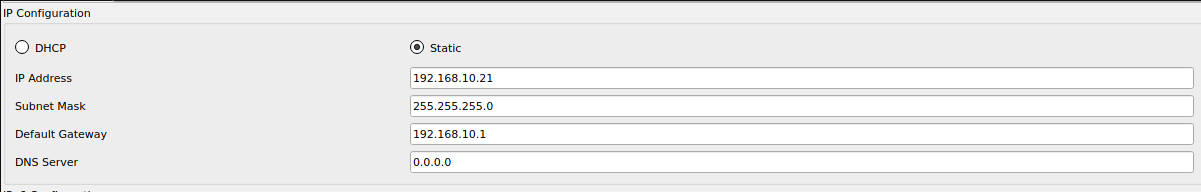
\includegraphics[width=.45\linewidth]{Figures/2020-03-18-165342_1201x192_scrot.png}}\hfill
\subfloat[IP config for
PC2]{\label{PC12PC2}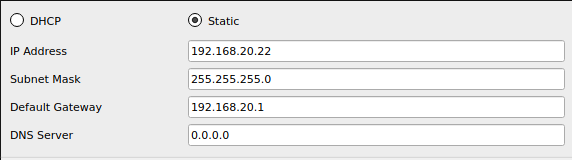
\includegraphics[width=.45\linewidth]{Figures/2020-03-18-165427_572x160_scrot.png}}\par 
\subfloat[IP config for
PC3]{\label{PC12PC3}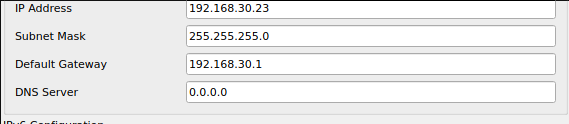
\includegraphics[width=.45\linewidth]{Figures/2020-03-18-165511_569x124_scrot.png}}\hfill
\subfloat[IP config for
PC4]{\label{PC12PC4}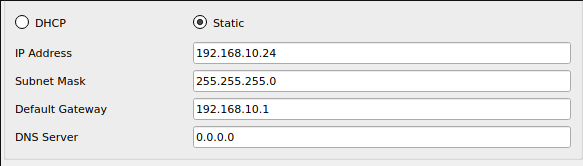
\includegraphics[width=.45\linewidth]{Figures/2020-03-18-165553_583x166_scrot.png}}\par
\subfloat[IP config for
PC5]{\label{PC12PC5}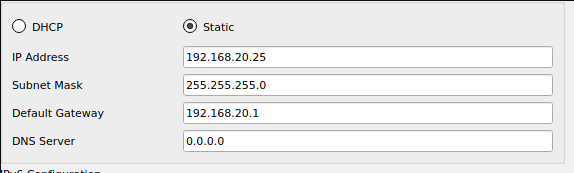
\includegraphics[width=.45\linewidth]{Figures/2020-03-18-165626_574x173_scrot.png}}\hfill
\subfloat[IP config for
PC6]{\label{PC12PC6}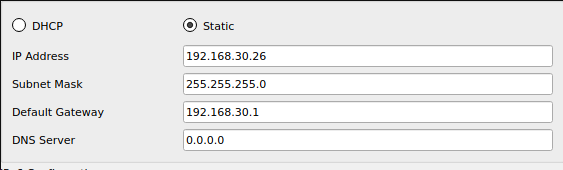
\includegraphics[width=.45\linewidth]{Figures/2020-03-18-165632_563x170_scrot.png}}\par
\caption{IP config for PC on the network}\label{PC12}
\end{figure}


\begin{figure}[!hbt]\centering
\subfloat[PC1 Pinging
PC4]{\label{Ping12PC1}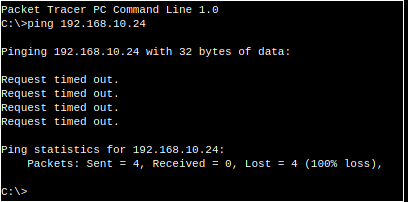
\includegraphics[width=.45\linewidth]{Figures/2020-03-18-165818_408x202_scrot.png}}\par
\subfloat[PC2 Pingin
PC5]{\label{Ping12PC2}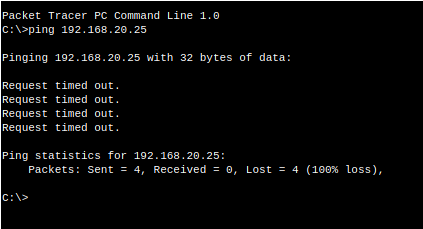
\includegraphics[width=.40\linewidth]{Figures/2020-03-18-165909_423x229_scrot.png}}\hfill 
\subfloat[PC3 Pingin
PC6]{\label{Ping12PC3}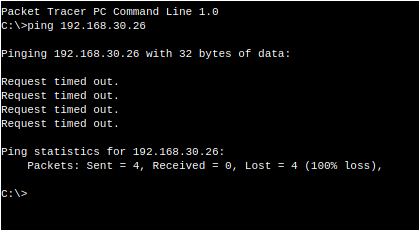
\includegraphics[width=.40\linewidth]{Figures/2020-03-18-170028_419x230_scrot.png}}\par
\caption{Pingin PCs on Joined Networks - Unsuccessfully}\label{Ping12}
\end{figure}

\clearpage

\noindent\mysubsection{2}{Verifying Switch Configuration}\\
In order to discover More about the switch configurations, and why the three
networks weren't able to communicate amongst themselves, I ran both
{\scriptsize{\verb$show ip int brief$}\normalsize}, see
Fig.~\ref{IP12} on Pg.~\pageref{IP12}. I then ran
{\scriptsize{\verb$show vlan brief$}\normalsize} on each of the switches, 
see Fig.~\ref{Vlan12} on Pg.~\pageref{Vlan12}.


\begin{figure}[!hbt]\centering
\subfloat[IP Brief on Switch 1]{\label{IP12S1}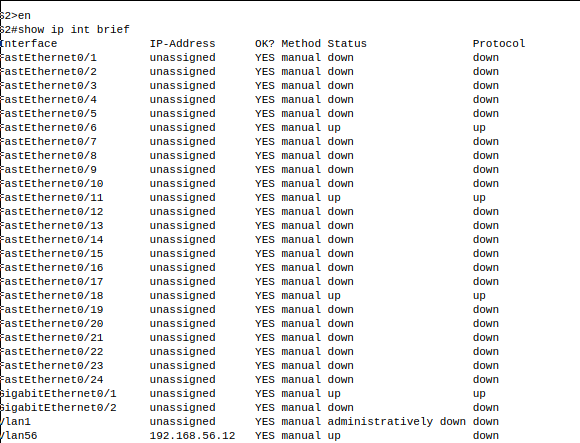
\includegraphics[width=.43\linewidth]{Figures/2020-03-18-225226_580x443_scrot.png}}\hfill
\subfloat[IP Brief on switch 3]{\label{IP12S3}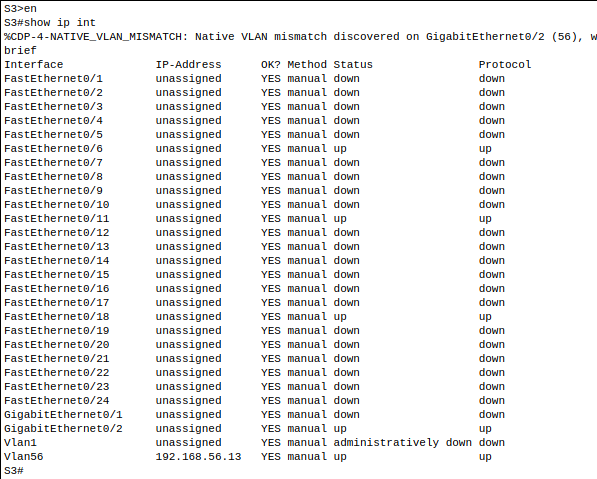
\includegraphics[width=.40\linewidth]{Figures/2020-03-18-225456_597x479_scrot.png}}\par
\subfloat[IP Brief on Switch 2]{\label{IP12S2}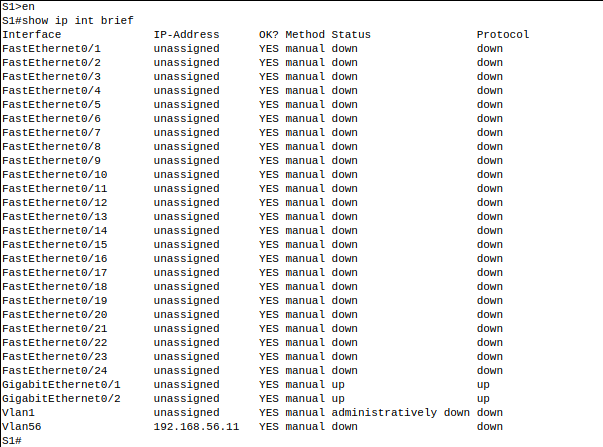
\includegraphics[width=.43\linewidth]{Figures/2020-03-18-225353_603x447_scrot.png}}\hfill 
\caption{Running show ip int brief on each switch}\label{IP12}
\end{figure}


\begin{figure}[!b]\centering
\subfloat[Vlan Brief on switch 2]{\label{Vlan12S2}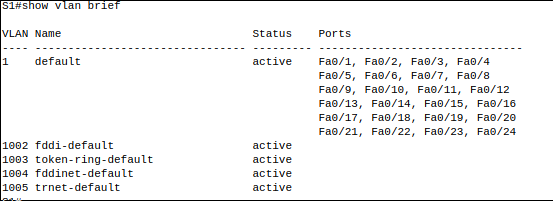
\includegraphics[width=.40\linewidth]{Figures/2020-03-18-225419_553x201_scrot.png}}\par 
\subfloat[Vlan Brief on Switch 1]{\label{Vlan12S1}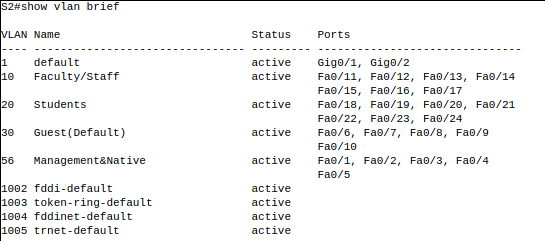
\includegraphics[width=.33\linewidth]{Figures/2020-03-18-225259_545x241_scrot.png}}\hfill
\subfloat[Vlan Brief on Switch 3]{\label{Vlan12S3}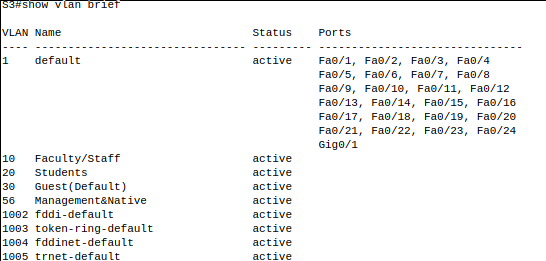
\includegraphics[width=.30\linewidth]{Figures/2020-03-18-225547_546x261_scrot.png}}
\caption{ Running show vlan brief on each switch }\label{Vlan12}
\end{figure}

\clearpage

\noindent\mysubsection{3}{Documenting the Problems and Solutions}\\
As you can see in Fig.~\ref{tab:Doc12} I have found the errors and will fix
them and then retest all of the connections.


\begin{table}[!h]
  \caption{Documentation}\label{tab:Doc12}
    \begin{tabular}{lp{0.45\linewidth}| lp{0.45\linewidth}p{1in}}
      \textbf{Problems} & \textbf{Solutions}\\\hline
      S1 not configured with any vlan & Configure Vlans\\
      S1 Native vlan 56 & set Native VLAN 56\\
      S2 g0/1 is an access port not a trunk port & Implement switchport mode\#
      trunk command\\
      s3 ports are not assigned to a VLAN & Implement switchport access vlan\#
      command based on the Port assignment table\\
    \end{tabular}
\end{table}


%===================================
\mysection{\textbf{Part 2: Implement Solutions and Test Connectivity}}

\mysubsection{1}{Setting up Switch 1}\\
For switch 1, I ran the following commands:

\begin{verbatim}
  en
conf t
vlan 56
name Management&Native
vlan 30
name Guest(Default)
vlan 10
name Faculty/Staff
vlan 20
name Students
int range g0/1 - 2
switchport trunk native vlan 56
\end{verbatim}

Once I ran those commands, I got the following in my tables:


\begin{figure}[!hbt]\centering
\subfloat[show ip int brief on S1]{\label{Show12S1Ip}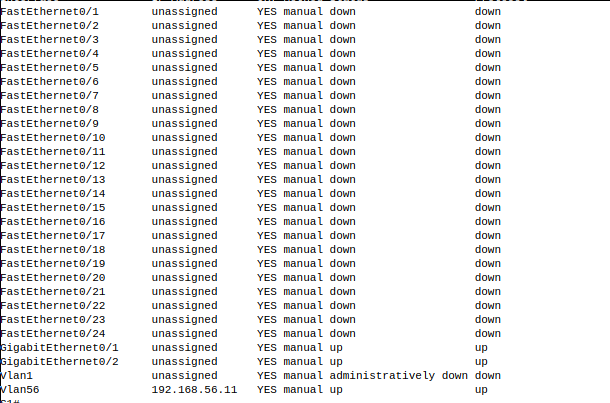
\includegraphics[width=.45\linewidth]{Figures/2020-03-19-160028_610x403_scrot.png}}\hfill
\subfloat[Show vlan brief on S1]{\label{Show12S1Vlan}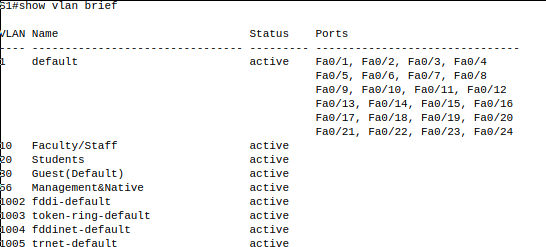
\includegraphics[width=.45\linewidth]{Figures/2020-03-19-160051_546x247_scrot.png}}\par 
\caption{S1 after configuration}
\label{Show12S1}
\end{figure}


\noindent\mysubsection{2}{Setting Up Switch 2}\\
For Switch 2, I ran the following commands:

\begin{verbatim}
  en
conf t
int g0/1
switchport mode trunk
\end{verbatim}

After running those commands, I got the following output:


\begin{figure}[!hbt]\centering
\subfloat[show ip int brief on S2]{\label{Show12S2Ip}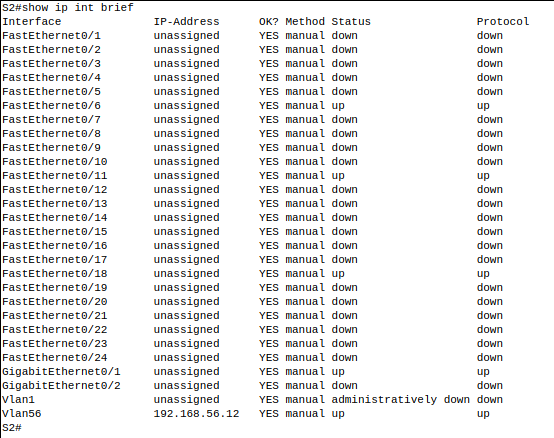
\includegraphics[width=.45\linewidth]{Figures/2020-03-19-160229_554x438_scrot.png}}\hfill
\subfloat[show vlan brief on S2]{\label{Show12S2Vlan}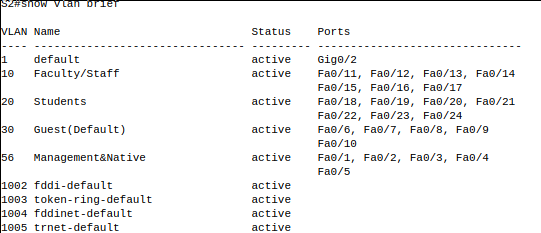
\includegraphics[width=.45\linewidth]{Figures/2020-03-19-160250_541x233_scrot.png}}\par 
\caption{S2 after configuration}
\label{Show12S2}
\end{figure}

\noindent\mysubsection{2}{Setting up Switch 3}\\
For switch 3, i ran the following commands:

\begin{verbatim}
  en
conf t
int range fa0/1 - 5
switchport access vlan 56
int range fa0/6 - 10
switchport access vlan 30
int range fa0/11 - 17
switchport access vlan 10
int range fa0/18 - 24
switchport access vlan 20
\end{verbatim}


\begin{figure}[!hbt]\centering
\subfloat[show ip int brief on S3]{\label{Show12S3Ip}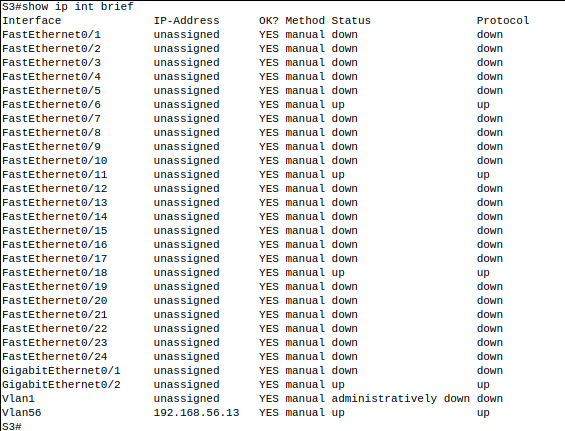
\includegraphics[width=.45\linewidth]{Figures/2020-03-19-160620_565x431_scrot.png}}\hfill
\subfloat[show vlan brief on S3]{\label{Show12S3Vlan}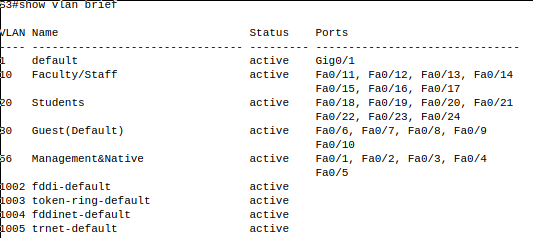
\includegraphics[width=.45\linewidth]{Figures/2020-03-19-160641_533x238_scrot.png}}\par 
\caption{Switch 3 after configuration}
\label{Show12S3}
\end{figure}


%===================================
\mysection{\textbf{Part 4: Conclusion}}
I was able to Ping each of the PCs within their connected networks, and I got
70/70 on the Scoring Rubric.


\begin{figure}[!hbt]\centering
\subfloat[PC1 pingin PC4]{\label{Conc12Ping1}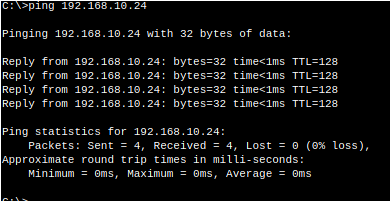
\includegraphics[width=.45\linewidth]{Figures/2020-03-19-162222_390x201_scrot.png}}\hfill
\subfloat[PC2 pingin PC5]{\label{Conc12Ping2}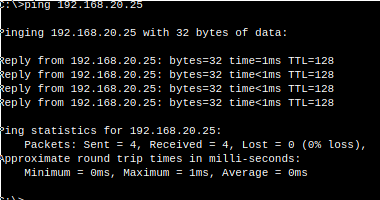
\includegraphics[width=.45\linewidth]{Figures/2020-03-19-162237_380x200_scrot.png}}\par
\subfloat[PC3 pingin PC6]{\label{Conc12Ping3}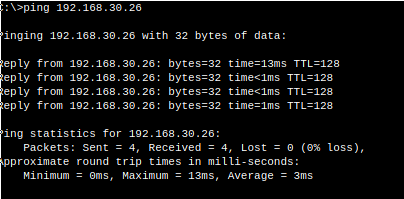
\includegraphics[width=.45\linewidth]{Figures/2020-03-19-162255_404x199_scrot.png}}\par
\subfloat[Final Score]{\label{Conc12Score}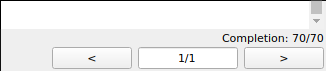
\includegraphics[width=.45\linewidth]{Figures/2020-03-19-162402_326x71_scrot.png}}\hfill
\caption{Pinging Networks and Final Score}
\label{Conc12}
\end{figure}

%===================================

\end{document}
